\documentclass[11pt]{article}

\usepackage[margin=1in]{geometry}
\usepackage[T1]{fontenc}
\usepackage{lmodern}
\usepackage{amsmath,amssymb}
\usepackage{booktabs}
\usepackage{graphicx}
\usepackage{xcolor}
\usepackage{tikz}
\usetikzlibrary{arrows.meta,positioning}
\usepackage[authoryear,round]{natbib}
\usepackage[colorlinks=true,linkcolor=blue!50!black,citecolor=blue!50!black,urlcolor=blue!50!black]{hyperref}

% Placeholder for numbers and findings that do not exist yet.
% Search the source for \todo before submitting.
\newcommand{\todo}[1]{\textnormal{\textcolor{red}{[TODO: #1]}}}

\newcommand{\um}{\,\ensuremath{\mu}m}
\newcommand{\nm}{\,nm}

\title{Optimizing Satellite Spectral Bands:\\[2pt]
\large Exact, Heuristic, and Differentiable Band Selection for\\
Land-Cover and Cloud Discrimination}
\author{Ryan Mohica\\GGS 426, Fall 2026}
\date{\todo{submission date}}

\begin{document}
\maketitle

\begin{abstract}
A multispectral sensor records a few bands out of the continuous 0.4--2.5\um{}
spectrum. We treat the choice of those bands as an optimization problem.
Candidate sensors are simulated from top-of-atmosphere (TOA) reflectance derived
from NASA EMIT imaging-spectrometer radiance, and band subsets are scored by the
worst-case Jeffries--Matusita (JM) distance among seven surface and cloud
classes. For $k \le 5$ bands we find the exact optimum of this score by
exhaustively evaluating every subset on a single workstation GPU, with the
search space split into resumable chunks through the combinatorial number
system. These optima
serve as ground truth for practical heuristics and for a differentiable model
that learns band centres and widths by gradient descent. The optimized designs
are compared with Landsat 8/9 OLI and the proposed Landsat Next.
\todo{one-sentence headline result for RQ1--RQ4.}
\end{abstract}

% ---------------------------------------------------------------------------
\section{Introduction}

Choosing where to place the bands of a multispectral sensor is usually done by
reasoning from reflectance curves: chlorophyll absorption in the red, the
leaf-scattering plateau in the near infrared, stronger ice absorption at
1.6\um, clay absorption near 2.2\um. That reasoning is sound but qualitative. It
cannot say whether a band set is the best possible, or how much each extra band
is worth. Data-driven optimization can answer both questions, provided the
results are checked against the physics.

We ask four research questions:
\begin{description}
  \item[RQ1.] For $k$ bands, which subset of EMIT bands maximises class
    separability, and how far below that optimum are Landsat 8/9 OLI and
    Landsat Next?
  \item[RQ2.] How close do practical heuristics come to the exact optimum, and
    how do they scale to larger $k$?
  \item[RQ3.] If band centres and widths are continuous design variables, where
    does gradient-based design place the bands, and is the placement physically
    interpretable?
  \item[RQ4.] How does throughput compare between a workstation GPU and the
    same machine's CPU, and how does CPU throughput scale with threads?
\end{description}

Throughout, ``exact optimum'' means the exact maximiser of the filter score
(Section~\ref{sec:objective}) on training-scene statistics. A classifier trained
on held-out scenes may rank subsets differently, so classifier results are
reported separately (Section~\ref{sec:evaluation}).

% ---------------------------------------------------------------------------
\section{Data}
\label{sec:data}

\paragraph{Imagery.} EMIT, on the International Space Station, records 285
bands from about 380 to 2500\nm{} at roughly 7.4\nm{} spacing and 60\,m pixels
\citep{green2020}. We use \todo{N} scenes covering contrasting biomes (desert,
cropland and grassland, forest, urban, coast), several of which contain liquid
and ice cloud. \todo{table of scene IDs, dates, locations.}

\paragraph{Top-of-atmosphere reflectance.} Surface-reflectance retrieval
assumes a clear view of the surface, which does not hold over clouds. To keep
every class on a common footing we start from the L1B radiance product and
convert each pixel to TOA reflectance,
\begin{equation}
  \rho_\mathrm{TOA}(\lambda) = \frac{\pi\, L(\lambda)\, d^2}{E_0(\lambda)\cos\theta_s},
  \label{eq:toa}
\end{equation}
where $L$ is at-sensor radiance, $d$ the Earth--Sun distance in AU,
$\theta_s$ the solar zenith angle, and $E_0$ the solar irradiance at 1\,AU.
$E_0$ is the TSIS-1 hybrid solar reference spectrum \citep{coddington2021},
averaged over each EMIT band with a Gaussian response of the band's published
full width at half maximum (FWHM). Fill values and pixels with the Sun at or
below the horizon are discarded.

\paragraph{Labels.} The seven classes are green vegetation, urban, bare
soil, sand, open water, liquid-water cloud, and ice cloud. Surface classes come
from ESA WorldCover 10\,m \citep{zanaga2022}. Each class is reprojected as a
0/1 layer with area averaging onto EMIT's orthorectified grid, giving the share
of every $\sim$60\,m cell it covers, and only cells at least 90\% covered by
one class are kept. Tree cover and grassland form the vegetation class;
shrubland and cropland are excluded because they mix vegetation and soil.
WorldCover has a single bare class, which is assigned to sand in desert scenes
and to bare soil elsewhere. Surface pixels must also carry no cloud, dilated
cloud, cirrus or spacecraft flag in the EMIT L2A mask. Cloud phase is labelled
by hand: polygons drawn from SWIR evidence (ice absorbs more strongly at
1.6\um) and visual interpretation mark liquid and ice cloud, and only pixels
inside a polygon that the L2A mask also flags as cloud are used.

Labels are built on the orthorectified grid and mapped back to sensor pixels
through EMIT's geometry lookup table, so spectra are never resampled. A sensor
pixel that receives two different labels is discarded. Up to 2000 pixels per
class and scene are sampled at random. \todo{pixel counts per class and scene.}

\paragraph{Reference sensors.} OLI and OLI-2 relative spectral responses
(USGS) and the published Landsat Next band edges \citep{usgs2024} are applied to
the EMIT spectra to produce baseline band sets.

% ---------------------------------------------------------------------------
\section{Methods}

\begin{figure}[t]
\centering
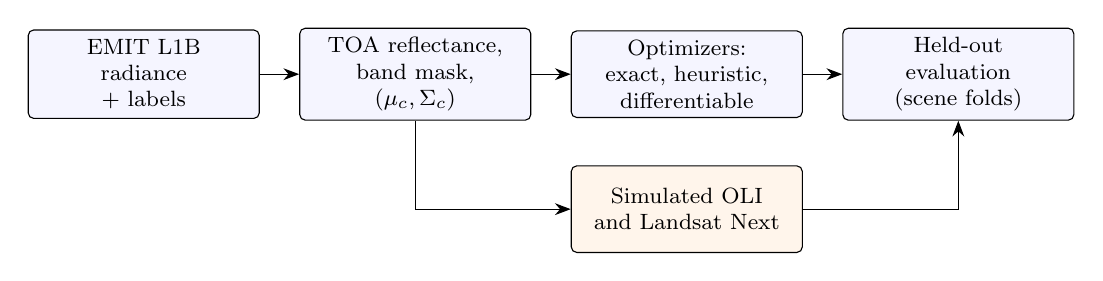
\begin{tikzpicture}[
    node distance=6mm and 5mm,
    box/.style={draw, rounded corners=2pt, align=center, font=\footnotesize,
                minimum height=11mm, text width=27mm, fill=blue!4},
    arr/.style={-{Stealth[length=2mm]}}]
  \node[box] (in) {EMIT L1B\\radiance\\+ labels};
  \node[box, right=of in] (toa) {TOA reflectance,\\band mask,\\$(\mu_c,\Sigma_c)$};
  \node[box, right=of toa] (opt) {Optimizers:\\exact, heuristic,\\differentiable};
  \node[box, right=of opt] (ev) {Held-out\\evaluation\\(scene folds)};
  \node[box, below=of opt, fill=orange!8] (ref) {Simulated OLI\\and Landsat Next};
  \draw[arr] (in) -- (toa);
  \draw[arr] (toa) -- (opt);
  \draw[arr] (opt) -- (ev);
  \draw[arr] (toa.south) |- (ref.west);
  \draw[arr] (ref.east) -| (ev.south);
\end{tikzpicture}
\caption{Workflow. Class statistics are computed from training scenes only.}
\label{fig:workflow}
\end{figure}

\subsection{Simulating sensors}

For a band $j$ with relative spectral response $s_j(\lambda)$, the simulated
band reflectance is
\begin{equation}
  \rho_j = \frac{\sum_\lambda s_j(\lambda)\,\rho(\lambda)\,\Delta\lambda}
                {\sum_\lambda s_j(\lambda)\,\Delta\lambda},
  \label{eq:simulate}
\end{equation}
with $\rho(\lambda)$ the EMIT TOA reflectance. We treat EMIT spacing as
uniform, so the $\Delta\lambda$ terms cancel.

\paragraph{Candidate bands.} Bands inside the strong water-vapour absorption
windows 1350--1420\nm{} and 1800--1950\nm{} are removed before the search,
leaving $n = \todo{n}$ candidates. The 1350--1420\nm{} window also holds OLI's
cirrus band, where ice cloud can remain bright while the surface is hidden. We
therefore run a sensitivity analysis for $k \le 4$ that keeps this window and
compares against the 8-band OLI set including cirrus; the main run compares
against the 7 reflective OLI bands.

\subsection{Class statistics}

Each class $c$ is summarised by its mean $\mu_c$ and covariance $\Sigma_c$ over
all candidate bands. Adjacent EMIT bands are highly correlated, so raw
covariances can be ill-conditioned. We use the Ledoit--Wolf shrinkage estimator
\citep{ledoit2004} and add a ridge of $10^{-6}$ times the mean variance to the
diagonal. Statistics are computed from training scenes only
(Section~\ref{sec:evaluation}).

\subsection{Objective}
\label{sec:objective}

For a subset $S$ of $k$ bands, let $\mu_{c,S}$ and $\Sigma_{c,S}$ be the
corresponding sub-vector and sub-matrix. The Bhattacharyya distance between
classes $a$ and $b$ is
\begin{equation}
  B_{ab}(S) = \tfrac{1}{8}(\mu_a-\mu_b)^\top \bar\Sigma^{-1}(\mu_a-\mu_b)
            + \tfrac{1}{2}\ln\frac{|\bar\Sigma|}{\sqrt{|\Sigma_a||\Sigma_b|}},
  \qquad \bar\Sigma = \tfrac12(\Sigma_a+\Sigma_b),
  \label{eq:bhatt}
\end{equation}
and the Jeffries--Matusita distance is $J_{ab} = 2(1-e^{-B_{ab}}) \in [0,2]$
\citep{richards2013}. The objective is worst-case separability,
\begin{equation}
  \max_{|S|=k} F(S), \qquad F(S) = \min_{a<b} J_{ab}(S),
  \label{eq:objective}
\end{equation}
so that no class pair is left confused.

Because $J$ is strictly increasing in $B$, maximising $\min_{a<b} B_{ab}$ gives
the same ranking as Eq.~\eqref{eq:objective}. We search on the Bhattacharyya
form because JM saturates near 2 and rounds many distinct subsets to the same
value in floating point. Subsets whose worst-case JM is within $0.001$ of the
best are treated as practical ties and ranked by mean pairwise JM.

\paragraph{Batched evaluation.} Both terms of Eq.~\eqref{eq:bhatt} come from
Cholesky factorisations: log-determinants from the factor diagonals, and the
Mahalanobis term from a triangular solve. Each subset needs one factorisation
per class and one per class pair (28 for seven classes), all of size
$k\times k$. General batched LAPACK and cuSOLVER routines carry per-call
overhead that dominates at this size, so we unroll the factorisation and the
forward substitution over the $k(k+1)/2$ lower-triangle entries. Each entry is
held as one contiguous tensor over all subsets and class pairs in the batch,
so every step is a single element-wise operation with sequential memory
access, and all class pairs are processed together. All arithmetic is in
double precision. A subset for which any factorisation meets a non-positive
pivot is marked as not scored rather than silently skipped.

\subsection{Exact search}
\label{sec:exact}

\begin{table}[t]
\centering
\caption{Size of the search space for $n = 255$ candidate bands. To be
recomputed from the final $n$.}
\label{tab:space}
\begin{tabular}{rrl}
\toprule
$k$ & $\binom{n}{k}$ & Approach \\
\midrule
3  & $2.7\times10^{6}$  & Exact, one GPU \\
4  & $1.7\times10^{8}$  & Exact, one GPU \\
5  & $8.6\times10^{9}$  & Exact, chunked and resumable \\
6  & $3.6\times10^{11}$ & Stretch goal \\
10 & $2.7\times10^{17}$ & Heuristics only \\
\bottomrule
\end{tabular}
\end{table}

Table~\ref{tab:space} gives the search-space sizes. Every subset is identified
by its rank in the combinatorial number system \citep{knuth2011}: a
$k$-subset $c_1<\dots<c_k$ has rank $\sum_{j=1}^{k}\binom{c_j}{j}$. The ranks
$[0,\binom{n}{k})$ are split into contiguous, near-equal chunks of about
$5\times10^7$ ranks. Within a chunk, ranks are unranked in batches of $10^5$
on the device (by a binary search over a precomputed table of binomial
coefficients for each position), scored, and merged into a running list of the
top 1000 subsets that stays in device memory. Each finished chunk is written to
disk at once, so an interrupted search resumes from the first missing chunk,
and disjoint chunk ranges can run on different machines and be merged
afterwards.

A merge step then verifies, before reporting any optimum, that
(i) the chunks cover the whole rank range with no gaps or overlaps,
(ii) every subset was scored successfully,
(iii) every chunk carries a fingerprint of the same statistics file, and
(iv) re-scoring the kept subsets from that file reproduces the stored
scores. Only a merge that passes all four checks is reported as an
exact optimum. It also flags when a chunk's top-1000 list may have truncated
near-ties, in which case the search is repeated with a larger list.

\subsection{Heuristics}
\todo{implementation pending; update once the code exists.}
For larger $k$ we evaluate sequential forward selection and sequential floating
forward selection \citep{pudil1994}, mRMR \citep{peng2005}, a genetic algorithm,
simulated annealing, and group-lasso multinomial logistic regression. The
stochastic methods run 30--50 seeds as independent array tasks. For $k$ where
the exact optimum $S^\star$ is known, each heuristic receives an optimality gap
$1 - F(S_\mathrm{heur})/F(S^\star)$.

\subsection{Differentiable sensor design}
\todo{implementation pending; update once the code exists.}
Each of the $k$ bands is modelled as a Gaussian response with learnable centre
$c_j$ and width $\sigma_j$,
\begin{equation}
  s_j(\lambda) = \exp\!\left[-\frac{(\lambda-c_j)^2}{2\sigma_j^2}\right],
  \label{eq:gaussian}
\end{equation}
applied through Eq.~\eqref{eq:simulate}. The band values feed a small neural
classifier trained end-to-end in PyTorch \citep{paszke2019}, following learned
filter design in imaging \citep{chakrabarti2016,nie2018}. The loss is
\begin{equation}
  \mathcal{L} = \mathcal{L}_\mathrm{CE}
    + \alpha \sum_j \frac{\sum_\lambda s_j(\lambda)A(\lambda)}{\sum_\lambda s_j(\lambda)}
    + \beta \sum_j \max\!\bigl(0,\, w_\mathrm{min} - 2.355\,\sigma_j\bigr)^2,
  \label{eq:loss}
\end{equation}
where $A(\lambda) = 1 - T(\lambda)$ is absorption from a standard-atmosphere
transmittance and $w_\mathrm{min}$ is a minimum FWHM. During training,
band-specific Gaussian noise with standard deviation proportional to
$1/\sqrt{\mathrm{FWHM}_j}$ models the dependence of SNR on bandwidth.

\subsection{Evaluation}
\label{sec:evaluation}

\paragraph{Leakage control.} Folds are whole scenes \citep{roberts2017}, and
every fold is required to contain training pixels of all seven classes. Class
statistics, and therefore band selection, use only a fold's training scenes;
selecting bands with held-out scenes would inflate held-out scores. Exact
search is run on every fold for $k\le4$ and on one fixed scene split for
$k=5$. A final run on all scenes is used only to report the selected bands,
never to score them.

\paragraph{Wrapper score.} Top subsets from each method are re-scored with
linear discriminant analysis, a random forest, and a small multilayer
perceptron, reporting macro-F1 and per-class F1 on held-out scenes.

\paragraph{Physical interpretation.} Each selected band is linked to an
absorption or scattering feature (chlorophyll, red edge, liquid water at 0.98
and 1.2\um, ice and liquid at 1.6\um, clay at 2.2\um). Selections that cannot
be explained physically are flagged as possible data artefacts.

\subsection{Implementation}

The code is Python, with batched scoring in PyTorch and scikit-learn for
covariance shrinkage and fold construction. The same code runs on a GPU or on
CPU threads. All runs use one workstation with an Intel Core i9
\todo{exact i9 model and RAM} and an NVIDIA GeForce RTX 5080 (16\,GB). A
benchmark script measures subsets per second on the GPU and on the CPU with
statistics of the planned size. Unit tests cover the unranking, the unrolled factorisation against
PyTorch's own, the separability scores against direct computation, resuming
and splitting a search, and the fold construction. The
repository, pinned environment, and job scripts reproduce every result.
\todo{repository URL and commit hash.}

% ---------------------------------------------------------------------------
\section{Results}

\subsection{RQ1: Exact optima and the Landsat gap}
\todo{Table: optimal subsets for $k=3,4,5$ (centre wavelengths), worst-case
and mean JM, per fold, with OLI and Landsat Next for comparison.}

\todo{Figure: selected band positions over the mean class TOA spectra.}

\todo{Cirrus sensitivity run, $k\le4$, against 8-band OLI.}

\subsection{RQ2: Heuristics versus the exact optimum}
\todo{Figure: optimality gap versus $k$ per method; spread across seeds.}

\subsection{RQ3: Learned band designs}
\todo{Learned centres and widths; comparison with exact subsets and Landsat Next.}

\subsection{RQ4: Scaling}
\todo{Measured subsets per second on the RTX 5080 and the i9 CPU for
$k=3$--6; speed-up and parallel efficiency against CPU thread count;
projected and measured wall time of the $k=5$ search.}

\subsection{Classifier evaluation}
\todo{Macro-F1 and per-class F1 on held-out scenes, focusing on liquid versus
ice cloud and urban versus soil/sand.}

% ---------------------------------------------------------------------------
\section{Discussion}
\todo{Physical interpretation of selected bands; agreement between filter and
wrapper rankings; stability across folds.}

\paragraph{Limitations.} WorldCover was mapped at 10\,m and in a different year
from some scenes, so labels carry noise despite the purity rule. TOA
reflectance includes atmospheric effects that vary between scenes, which the
filter score treats as class variance. The exact optimum is optimal only for
the Gaussian-class filter score on training statistics, not for any particular
classifier. \todo{further limitations from the results.}

% ---------------------------------------------------------------------------
\section{Conclusion}
\todo{Answer to each research question in one or two sentences.}

\bibliographystyle{plainnat}
\bibliography{refs}

\end{document}
